In this section, the processing unit layer is described in some detail in terms of its specific subsystems. The processing unit comprises two primary components: the host PC and the Raspberry Pi. This layer plays a crucial role in the robotic system by acquiring input data from sensors and processing it before transmitting the processed data to the robot controllers.

\subsection{Host PC}
The host PC acts as a powerful processing unit for in-depth analysis, decision making, and control. It receives pre-processed data from the Raspberry Pi, including data from the QR code, and it performs trajectory planning and higher level decision making.

\begin{figure}[h!]
	\centering
 	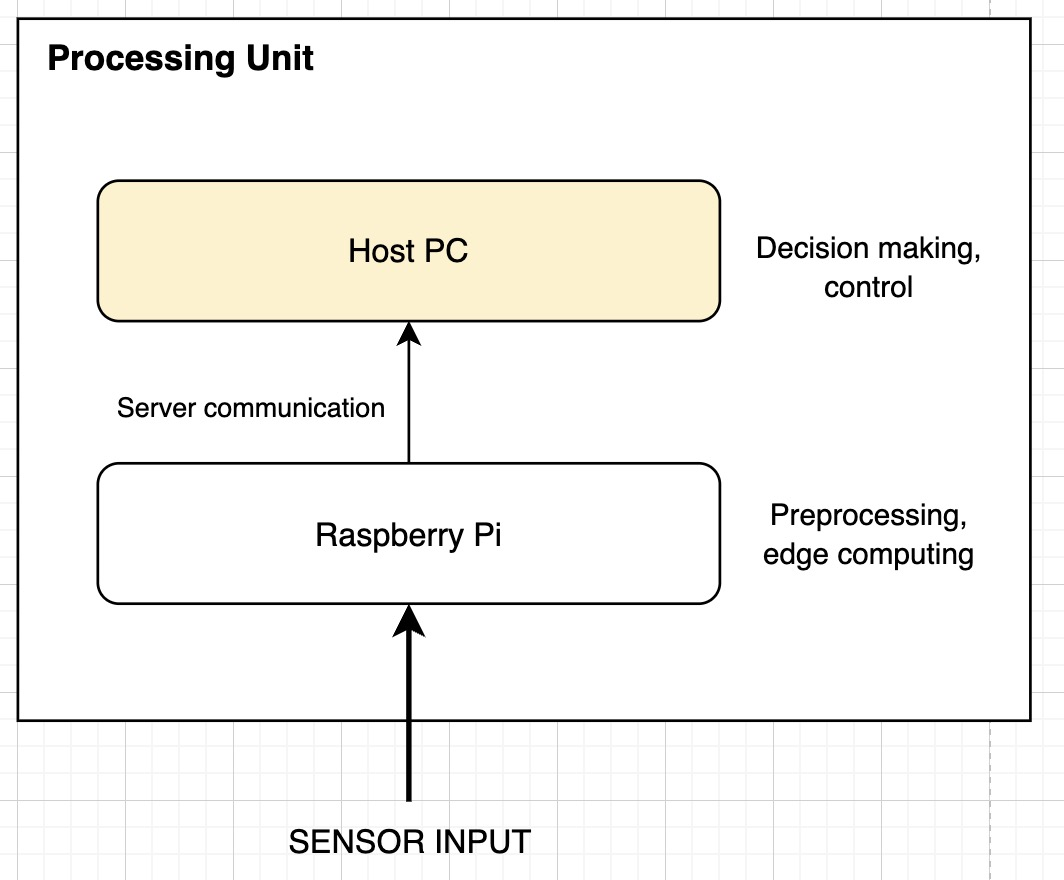
\includegraphics[width=0.60\textwidth]{images/host_pc.png}
 \caption{Host PC subsystem}
\end{figure}

\subsubsection{Assumptions}
\begin{itemize}
    \item The host PC assumes a stable connection to the Raspberry Pi for data transfer.
    \item The host PC assumes that data received from Raspberry Pi is processed correctly.
\end{itemize}
\subsubsection{Responsibilities}
\begin{itemize}
    \item Data Analysis: The host PC is responsible for analyzing the data received from the Raspberry Pi, which includes processing sensor data, decoding QR codes, and running various algorithms for object recognition.
    \item Decision-Making: Based on the data analysis, the host PC is responsible for making high-level decisions, such as robot control commands, path planning, and task scheduling.
    \item Communication with PLC: The host PC is responsible for communicating with the Programmable Logic Controller (PLC) to issue control commands and receive status updates.
    \item Output to Indicators: The host PC is responsible for sending instructions to indicators to provide visual feedback to operators.
\end{itemize}

\subsubsection{Subsystem Interfaces}

\begin {table}[H]
\caption {Subsystem interfaces} 
\begin{center}
    \begin{tabular}{ | p{1cm} | p{6cm} | p{4cm} | p{4cm} |}
    \hline
    ID & Description & Inputs & Outputs \\ \hline
    \#01 & Data input from Raspberry Pi & \pbox{4cm}{Preprocessed sensor data \\ QR code results } & \pbox{4cm}{Control instructions}  \\ \hline
    \#02 & Communication with PLC & \pbox{3cm}{N/A} & \pbox{4cm}{Control commands}  \\ \hline
    \end{tabular}
\end{center}
\end{table}

\subsection{Raspberry Pi}
The Raspberry Pi serves as an integral component of the processing unit within the robot system. It fulfills the role of an edge computing device, responsible for initial data processing and interfacing between the sensors and the host PC. Specifically, the Raspberry Pi is responsible for collecting data from a variety of sensors, including those for QR code scanning and other environmental monitoring.
\begin{figure}[h!]
	\centering
 	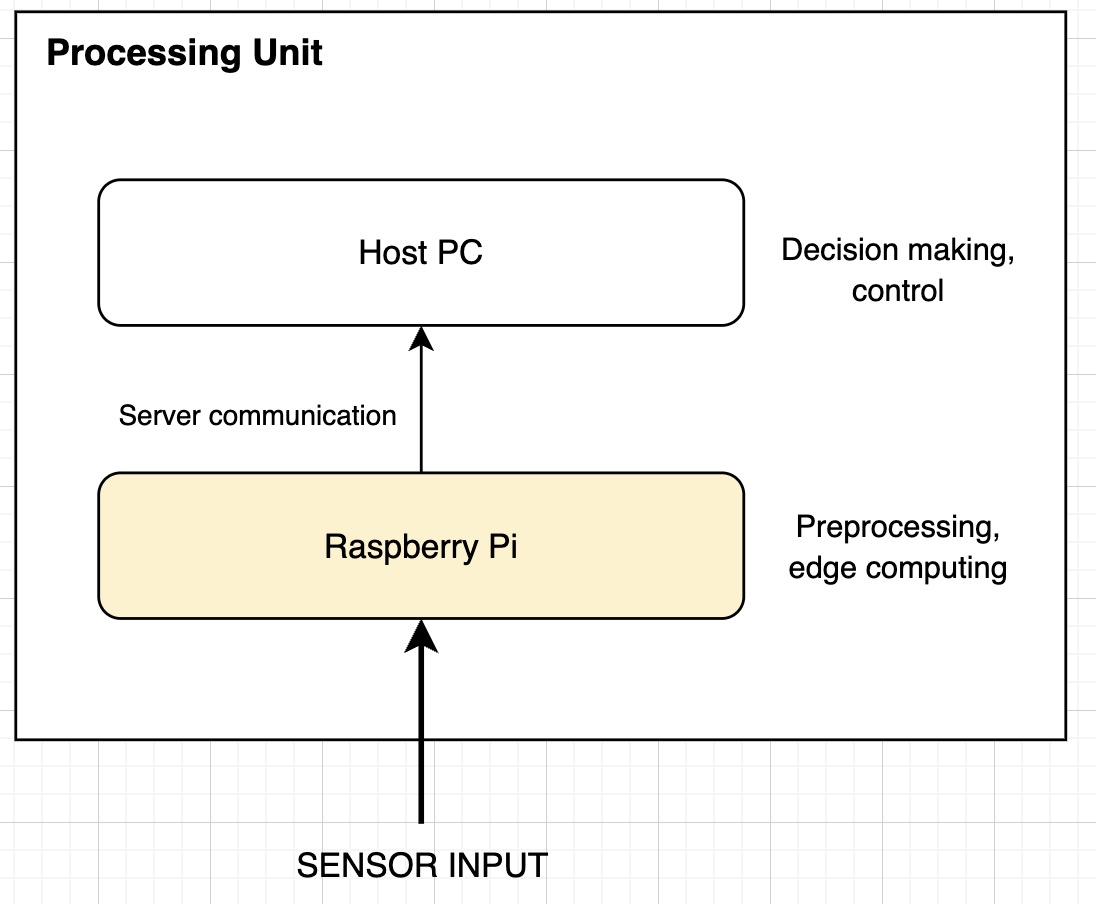
\includegraphics[width=0.60\textwidth]{images/rpi.png}
 \caption{Raspberry Pi subsystem}
\end{figure}

\subsubsection{Assumptions}
\begin{itemize}
    \item The Raspberry Pi is properly installed on the robot arm and receives sensor input data correctly.
    \item The Raspberry Pi receives data in the expected format.
    \item The Raspberry Pi has the necessary software and libraries installed for data preprocessing.
    \item The Raspberry Pi has an established connection with the Raspberry Pi.
\end{itemize}
\subsubsection{Responsibilities}
\begin{itemize}
    \item Sensor Data Collection: The Raspberry Pi is responsible for collecting data from various sensors, such as cameras and QR code scanners.
    \item Data Preprocessing: The Raspberry Pi preprocesses the collected data, which may include image processing, decoding QR codes, and initial data filtering.
    \item Data Transfer: It is responsible for transferring the preprocessed data to the host PC for further analysis and decision-making.
\end{itemize}

\subsubsection{Subsystem Interfaces}

\begin {table}[H]
\caption {Subsystem interfaces} 
\begin{center}
    \begin{tabular}{ | p{1cm} | p{6cm} | p{4cm} | p{4cm} |}
    \hline
    ID & Description & Inputs & Outputs \\ \hline
    \#01 & Sensor data & \pbox{4cm}{Sensor data streams} & \pbox{4cm}{Preprocessed data}  \\ \hline
    \#02 & Communication with host PC & \pbox{4cm}{N/A} & \pbox{4cm}{Data to be analyzed}  \\ \hline
    \end{tabular}
\end{center}
\end{table}


